\documentclass[11pt,compress,t,notes=noshow]{beamer}\usepackage[]{graphicx}\usepackage[]{color}

\makeatletter
\def\maxwidth{ %
  \ifdim\Gin@nat@width>\linewidth
    \linewidth
  \else
    \Gin@nat@width
  \fi
}
\makeatother

\definecolor{fgcolor}{rgb}{0.345, 0.345, 0.345}
\newcommand{\hlnum}[1]{\textcolor[rgb]{0.686,0.059,0.569}{#1}}%
\newcommand{\hlstr}[1]{\textcolor[rgb]{0.192,0.494,0.8}{#1}}%
\newcommand{\hlcom}[1]{\textcolor[rgb]{0.678,0.584,0.686}{\textit{#1}}}%
\newcommand{\hlopt}[1]{\textcolor[rgb]{0,0,0}{#1}}%
\newcommand{\hlstd}[1]{\textcolor[rgb]{0.345,0.345,0.345}{#1}}%
\newcommand{\hlkwa}[1]{\textcolor[rgb]{0.161,0.373,0.58}{\textbf{#1}}}%
\newcommand{\hlkwb}[1]{\textcolor[rgb]{0.69,0.353,0.396}{#1}}%
\newcommand{\hlkwc}[1]{\textcolor[rgb]{0.333,0.667,0.333}{#1}}%
\newcommand{\hlkwd}[1]{\textcolor[rgb]{0.737,0.353,0.396}{\textbf{#1}}}%
\let\hlipl\hlkwb

\usepackage{framed}
\makeatletter
\newenvironment{kframe}{%
 \def\at@end@of@kframe{}%
 \ifinner\ifhmode%
  \def\at@end@of@kframe{\end{minipage}}%
  \begin{minipage}{\columnwidth}%
 \fi\fi%
 \def\FrameCommand##1{\hskip\@totalleftmargin \hskip-\fboxsep
 \colorbox{shadecolor}{##1}\hskip-\fboxsep
     \hskip-\linewidth \hskip-\@totalleftmargin \hskip\columnwidth}%
 \MakeFramed {\advance\hsize-\width
   \@totalleftmargin\z@ \linewidth\hsize
   \@setminipage}}%
 {\par\unskip\endMakeFramed%
 \at@end@of@kframe}
\makeatother

\definecolor{shadecolor}{rgb}{.97, .97, .97}
\definecolor{messagecolor}{rgb}{0, 0, 0}
\definecolor{warningcolor}{rgb}{1, 0, 1}
\definecolor{errorcolor}{rgb}{1, 0, 0}
\definecolor{code}{rgb}{0.97, 0.96, 1.0}
\newenvironment{knitrout}{}{} % an empty environment to be redefined in TeX

\usepackage{alltt}
\usepackage[utf8]{inputenc}
\usepackage[ngerman]{babel}
\usepackage{dsfont}
\usepackage{verbatim}
\usepackage{amsmath}
\usepackage{amsfonts}
\usepackage{mathtools}
\usepackage{csquotes}
\usepackage{cmbright}
\usepackage{multirow}
\usepackage{longtable}
\usepackage{enumerate}
\usepackage[absolute,overlay]{textpos}
\usepackage{psfrag}
\usepackage{algorithm}
\usepackage{algpseudocode}
\usepackage{eqnarray}
\usepackage{bytefield}
\usepackage{animate}
\usepackage{tikz}
\usetikzlibrary{shapes,matrix,positioning,chains,arrows,shadows,decorations.pathmorphing,fit,backgrounds}
\usepackage{adjustbox}
\usepackage{colortbl}
\usepackage{tabularx} % for tables (incl. \hline)
\usepackage{arydshln} % Load after array, longtable, colortab and/or colortbl , otherwise problems with \hline in tabular env
\usepackage{etex} %increase registers for \dimenS to more than 256, otherwise we get "No room for a new \dimen"
\usepackage{graphicx}
\usepackage{booktabs} %used in epr lectures
\usepackage{bm} % bold greek letters
\usepackage{hyperref} % url citing
\usepackage{blkarray} % block arrays
\usepackage{listings} % block of code
\usepackage{xcolor} %colored math symbols
\usepackage{pgffor}
\usepackage{verbatimbox}
\usepackage{xcolor}

%some colors
\definecolor{checkgreen}{HTML}{18A126}
\definecolor{errorred}{HTML}{FF0000}
\definecolor{blockbg}{HTML}{F7F7F7}
\definecolor{gray}{HTML}{A0A0A0}

% basic latex stuff
\newcommand{\col}{\par\colorbox{code}{\parbox{\textwidth}{\theverbbox}}\par}
\newcommand{\eg}{e.\,g.\xspace} %for example
\newcommand{\ie}{i.\,e.\xspace} %that is to say...
\newcommand{\pkg}[1]{{\fontseries{b}\selectfont #1}} %fontstyle for R packages
\newcommand{\lz}{\vspace{0.5cm}} %vertical space
\newcommand{\oneliner}[1] % Oneliner for important statements
{\begin{block}{}\begin{center}\begin{Large}#1\end{Large}\end{center}\end{block}}
\def\SpAr{\quad \Rightarrow \quad}

%new environments
\newenvironment{vbframe}  %frame with breaks and verbatim
{
 \begin{frame}[containsverbatim,allowframebreaks]
}
{
\end{frame}
}

\newenvironment{vframe}  %frame with verbatim without breaks (to avoid numbering one slided frames)
{
 \begin{frame}[containsverbatim]
}
{
\end{frame}
}

\newenvironment{blocki}[1]   % itemize block
{
 \begin{block}{#1}\begin{itemize}
}
{
\end{itemize}\end{block}
}

\newenvironment{fragileframe}[2]{  %fragile frame with framebreaks
\begin{frame}[allowframebreaks, fragile, environment = fragileframe]
\frametitle{#1}
#2}
{\end{frame}}

\newcommand{\myframe}[2]{  %short for frame with framebreaks
\begin{frame}[allowframebreaks]
\frametitle{#1}
#2
\end{frame}}

\usepackage{../../style/lmu-lecture}

\let\code=\texttt
\let\proglang=\textsf

\setkeys{Gin}{width=0.9\textwidth}

\usepackage{tikz}
\usetikzlibrary{shapes,arrows,snakes, calc}

% Define block styles
\tikzstyle{decision} = [diamond, draw, text width=6em, text badly centered, node distance=4cm, inner sep=0pt]
\tikzstyle{decision2} = [diamond, draw, fill=customgreen!35, text width=6em, text badly centered, node distance=4cm, inner sep=0pt]

\tikzstyle{block} = [rectangle, draw, text width=14em, text centered, rounded corners, node distance=3cm, minimum height=4em]
\tikzstyle{line} = [draw, -latex']
\tikzstyle{cloud} = [draw, ellipse, node distance=3cm, minimum height=2em]

\title{Introduction to Deep Learning}
\author{Bernd Bischl}
\institute{Department of Statistics -- LMU Munich}
\date{WS 2021/2022}

\setbeamertemplate{frametitle}{\expandafter\uppercase\expandafter\insertframetitle}

\IfFileExists{upquote.sty}{\usepackage{upquote}}{}
\input{../../latex-math/basic-math}
\input{../../latex-math/basic-ml}
\input{../../latex-math/ml-nn}

\begin{document}
\newcommand{\titlefigure}{figure/alexnetfront.png}
%modify picture
\newcommand{\learninggoals}{
  \item Application of CNNs in Visual Recognition
}

\lecturechapter{CNN Applications}
\lecture{I2DL}

%%%%%%%%%%%%%%%%%%%%%%%%%%%%%%%%%%%%%%%%%%%%%%%%%%%%%%%%%%%%%%%%%%
\begin{vbframe}{Application - Image Classification}
    \begin{itemize}
        \item One of use case for the CNNs is image classification.
        \item There exists a broad variety of network architectures for image classification such as the LeNet, AlexNet, InceptionNet and ResNet which will be discussed in detail in the next lecture.
        \item All these architectures rely on a set of a sequence of convolutional layers and aim to learn the mapping from an image to a probability score over a set of classes.
    \end{itemize}
\framebreak
    \begin{figure}
        \centering
        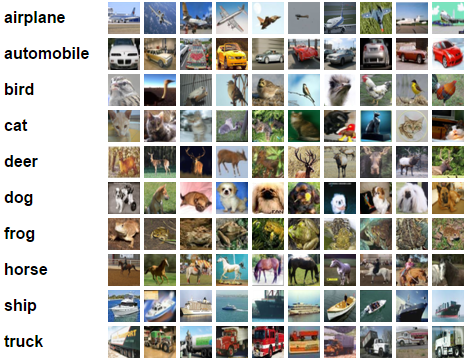
\includegraphics[width=7cm]{figure/recognition.png}
        \caption{Image classification with Cifar 10: famous benchmark dataset with 60000 images and 10 classes (Alex Krizhevsky (2009)). There is also a much more difficult version with 60000 images and 100 classes.}
    \end{figure}
\framebreak
    \begin{figure}
        \centering
        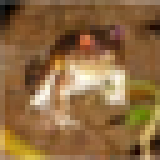
\includegraphics[width=4cm]{figure/cifar_frog.png}
        \caption{One example of the Cifar10 data: A highly pixelated, coloured image of a frog with dimension [3, 32, 32]. }
    \end{figure}
\framebreak
    \begin{figure}
        \centering
          \scalebox{1}{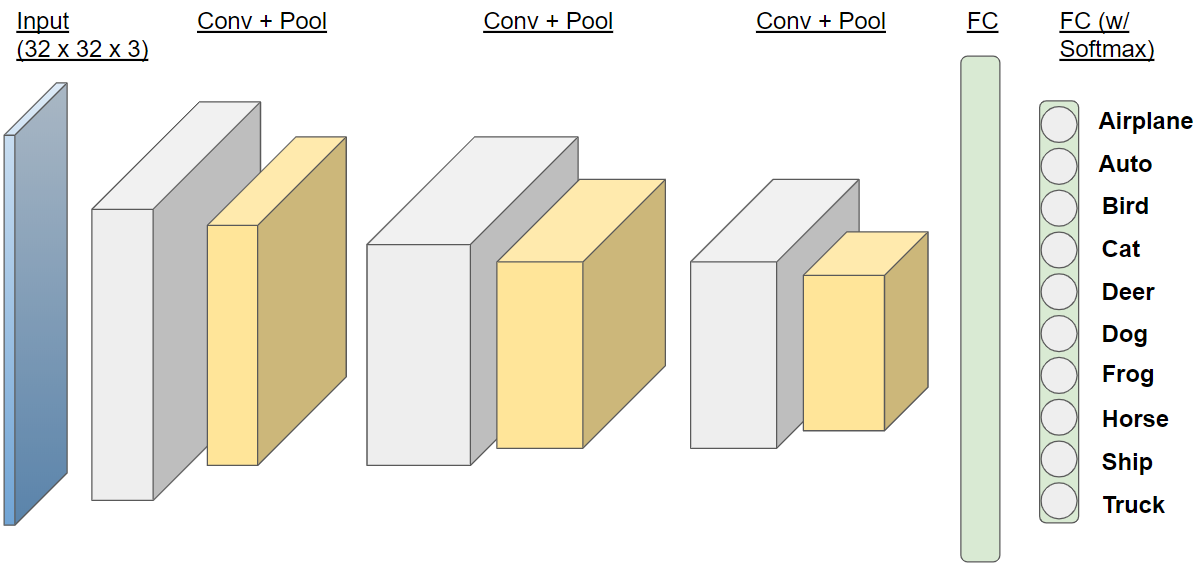
\includegraphics{figure/cifar10_eg.png}}
        \caption{An example of a CNN architecture for classification on the Cifar10 dataset (FC = Fully Connected). }
    \end{figure}  
\end{vbframe}

\begin{frame} {CNN vs a Fully Connected net on Cifar10}
  \begin{figure}
        \centering
          \scalebox{0.75}{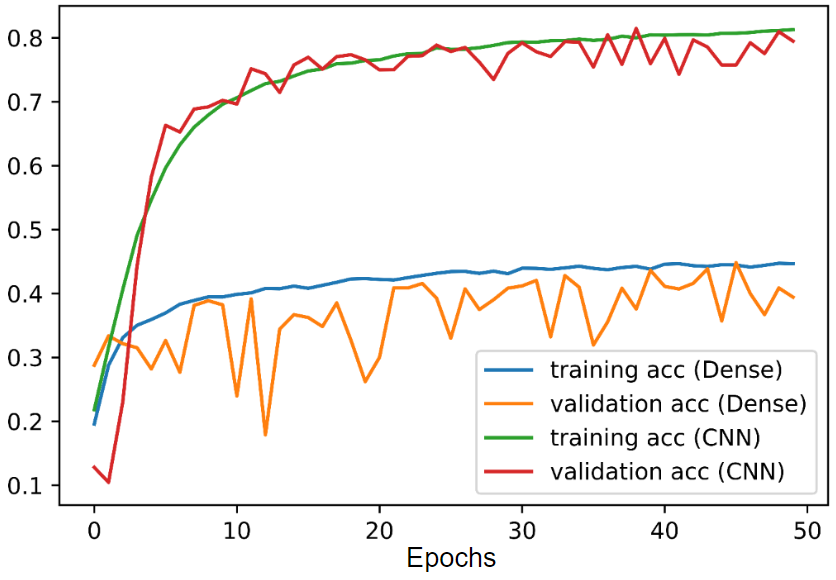
\includegraphics{figure/cnn_vs_dense_1.png}}
        \caption{Performance of a CNN and a fully connected neural net ("Dense") on Cifar-10. Both networks have roughly the same number of layers. They were trained using the same learning rate, weight decay and dropout rate. Of course, the CNN performs better because it has less learnable parameters and the right inductive bias for the task.}
    \end{figure} 
\end{frame}
%%%%%%%%%%%%%%%%%%%%%%%%%%%%%%%%%%%%%%%%%%%%%%%%%%%%%%%%%%%%%%%%%%
\begin{vbframe}{Application - Beyond Image Classification}
There are many visual recognition problems that are related to image classification, such as:

\begin{itemize}
    \item object detection
    \item image captioning
    \item semantic segmentation
    \item visual question answering
    \item visual instruction navigation
    \item scene graph generation
\end{itemize}
\end{vbframe}


\begin{vbframe}{Application - Image Colorization}
    \begin{itemize}
        \item Basic idea (introduced by Zhang et al., 2016):
        \begin{itemize}
            \item Train the net on pairs of grayscale and coloured images.
            \item Force it to make a prediction on the colour-value \textbf{for each pixel} in the grayscale input image.
            \item Combine the grayscale-input with the colour-output to yield a colorized image.
        \end{itemize}
        \item Very comprehensive material on the method is provided on the author's website. \href{http://richzhang.github.io/colorization/}{\beamergotobutton{Click here}}
            \end{itemize}
            \framebreak
            \begin{figure}
            \centering
            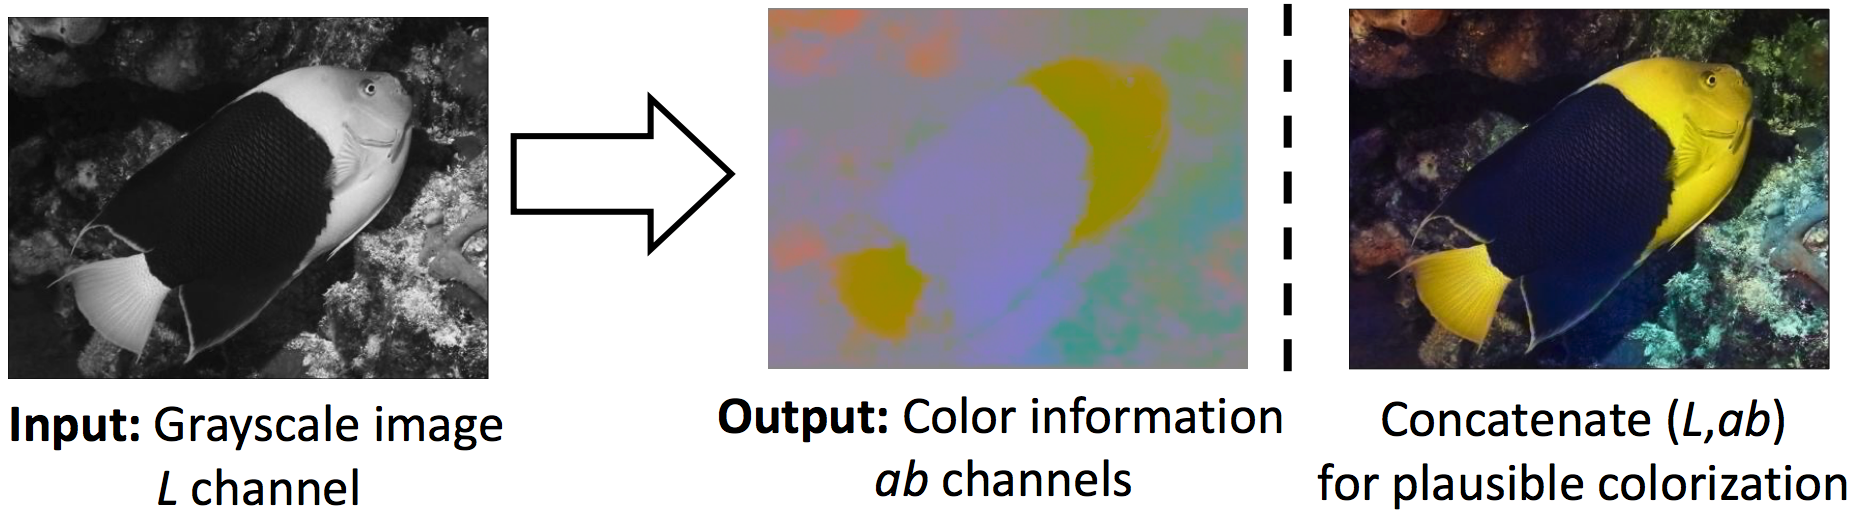
\includegraphics[width=11cm]{figure/fish_lab.png}
            \caption{The CNN learns the mapping from grayscale (L) to color (ab) for each pixel in the image. The L and ab maps are then concatenated to yield the colorized image. The authors use the LAB color space for the image representation.}
            \end{figure}
            \framebreak
            \begin{figure}
            \centering
            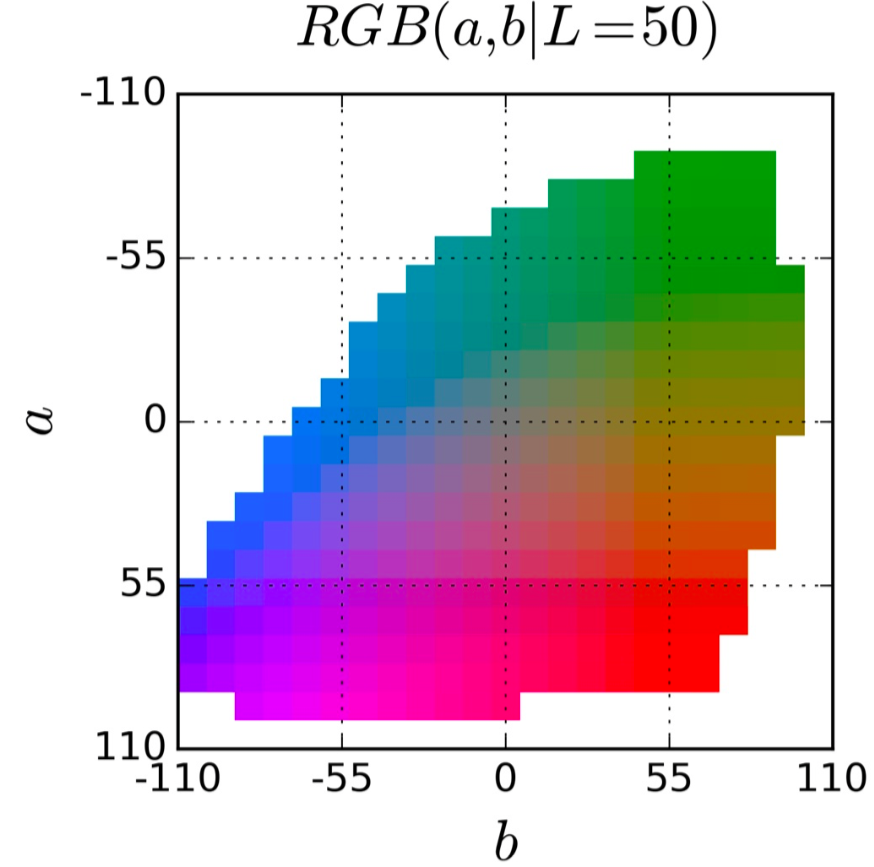
\includegraphics[width=5cm]{figure/lab.png}
            \caption{The colour space (ab) is quantized in a total of 313 bins. This allows to treat the color prediction as a classification problem where each pixel is assigned a probability distribution over the 313 bins and that with the highest softmax-score is taken as predicted color value. The bin is then mapped back to the corresponding, numeric (a,b) values. The network is optimized using a multinomial cross entropy loss over the 313 quantized (a,b) bins.}
            \end{figure}
            \framebreak
            \begin{figure}
            \centering
            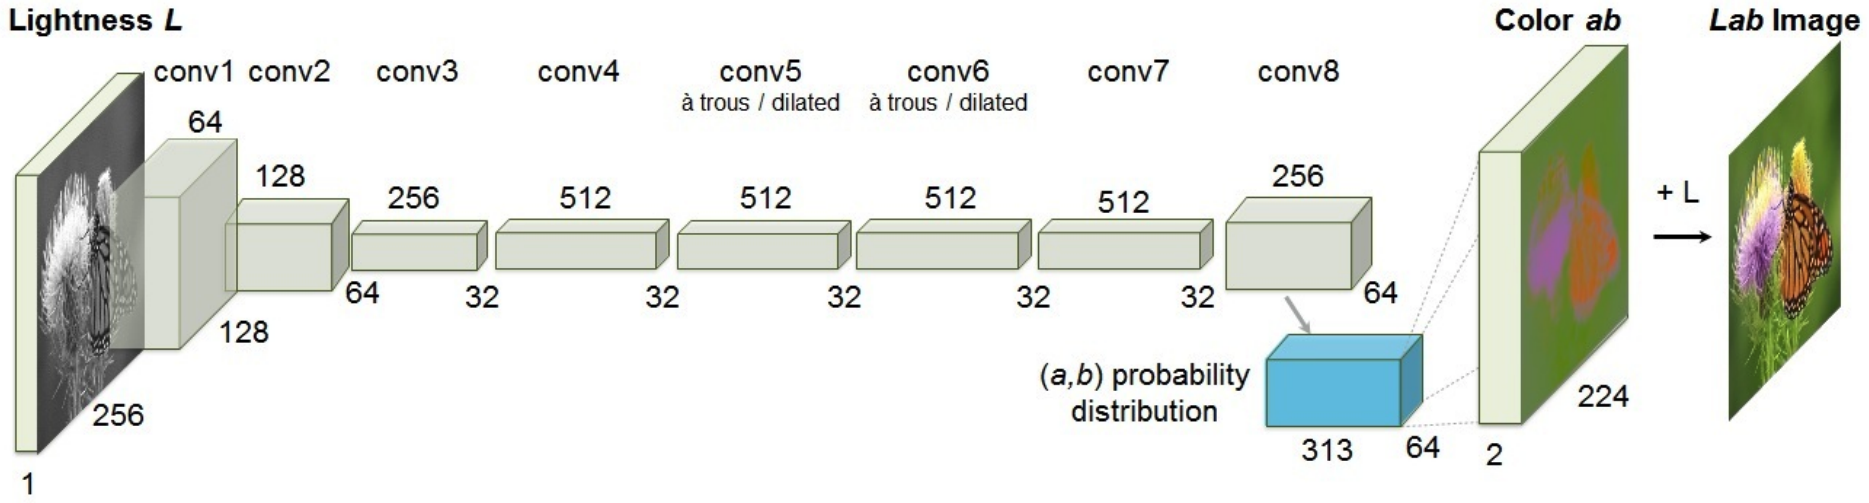
\includegraphics[width=11.5cm]{figure/color_architecture.png}
            \caption{The architecture consists of stacked CNN layers which are upsampled towards the end of the net. It makes use of \textit{dilated convolutions} and \textit{upsampling layers} which are explained in the next lecture. The output is a tensor of dimension [64, 64, 313] that stores the 313 probabilities for each element of the final, downsampled 64x64 feature maps.} 
            \end{figure}
            \framebreak
            \begin{figure}
            \centering
            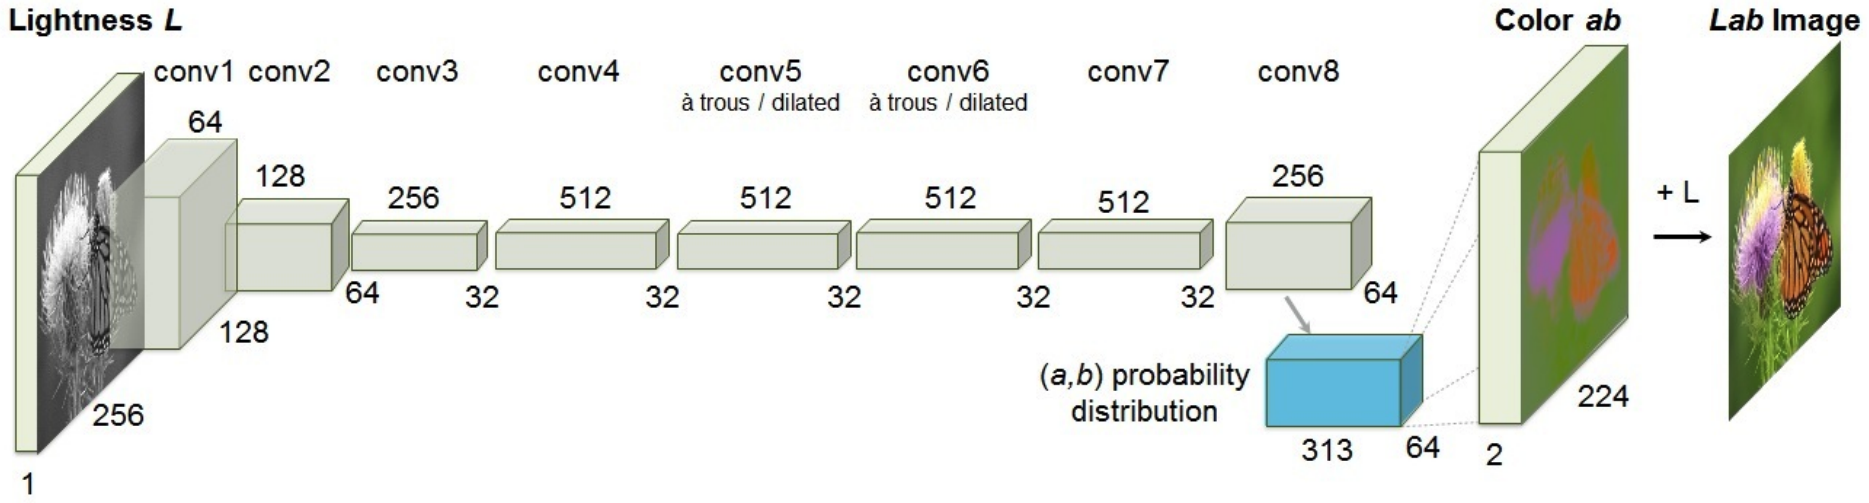
\includegraphics[width=11.5cm]{figure/color_architecture.png}
            \caption{This block is then upsampled to a dimension of 224x224 and the predicted color bins are mapped back to the (a,b) values yielding a depth of 2. Finally, the L and the ab maps are concatenated to yield a colored image.} 
            \end{figure}
            \end{vbframe}
            %%%%%%%%%%%%%%%%%%%%%%%%%%%%%%%%%%%%%%%%%%%%%%%%%%%%%%%%%%%%%%%%%%
                %%%%%%%%%%%%%%%%%%%%%%%%%%%%%%%%%%%%%%%%%%%%%%%%%%%%%%%%%%%%%%%%%%
                \begin{vbframe}{Application - Object localization}
            \begin{itemize}
            \item Until now, we used CNNs for \textit{single}-class classification of images - \textbf{which object is on the image?}
            \item Now we extend this framework - \textbf{is there an object in the image and if yes, where and which?}
            \end{itemize}
            \begin{figure}
            \centering
            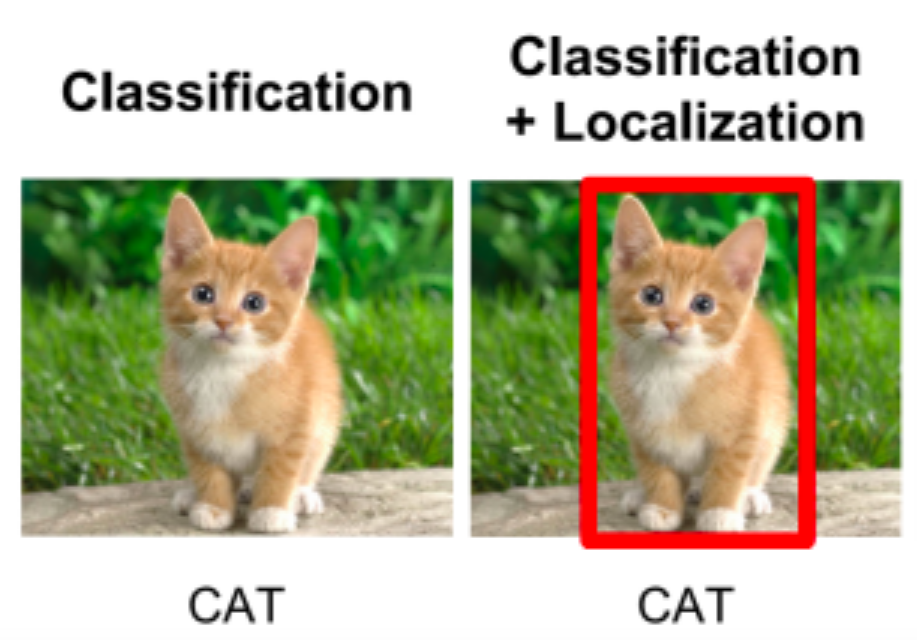
\includegraphics[width=4cm]{figure/localize_cat.png}
            \caption{Classify and detect the location of the cat.}
            \end{figure}
            \framebreak
            \begin{itemize}
            % source1:  https://medium.com/machine-learning-bites/deeplearning-series-objection-detection-and-localization-yolo-algorithm-r-cnn-71d4dfd07d5f
            % source2: https://leonardoaraujosantos.gitbooks.io/artificial-inteligence/content/object_localization_and_detection.html
            \item Bounding boxes can be defined by the location of the left lower corner as well as the height and width of the box: [$b_x$, $b_y$, $b_h$, $b_w$].
            \item We now combine three tasks (detection, classification and localization) in one architecture.
            \item This can be done by adjusting the label output of the net.
            \item Imagine a task with three classes (cat, car, frog).
            \item In standard classification we would have: 
                $$
                \text{label vector}
            \begin{bmatrix}
            c_{cat}\\
            c_{car} \\
            c_{frog}
            \end{bmatrix}
            \text{and softmax output}
            \begin{bmatrix}
            P(y = cat| X, \theta)\\
            P(y = car| X, \theta)\\
            P(y = frog| X, \theta)
            \end{bmatrix}
            $$
                \end{itemize}
            \framebreak
            \begin{itemize}
            \item We include the information, if there is a object as well as the bounding box parametrization in the label vector.
            \item This gives us the following label vector:
                $$
                \begin{bmatrix}
            b_x\\
            b_y \\
            b_h \\
            b_w.\\
            c_o \\
            c_{cat} \\
            c_{car} \\
            c_{frog} \\
            \end{bmatrix} =             
                \begin{bmatrix}
            \text{x coordinate box}\\
            \text{y coordinate box} \\
            \text{height box} \\
            \text{width box}.\\
            \text{presence of object, binary} \\
            \text{class cat, one-hot} \\
            \text{class car, one-hot}\\
            \text{class frog, one-hot} \\
            \end{bmatrix}
            $$
                \end{itemize}
            \framebreak
            \begin{figure}
            \centering
            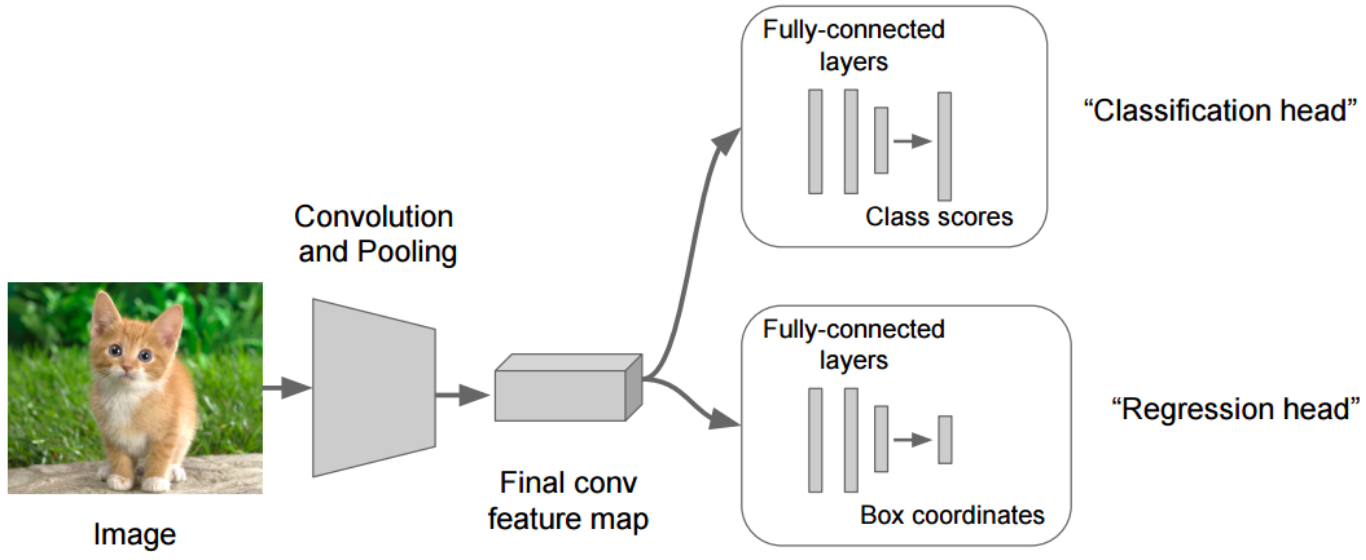
\includegraphics[width=8cm]{figure/naive_localization.png}
            \end{figure}
            \begin{itemize}
            \item Naive approach: use a CNN with two heads, one for the class classification and one for the bounding box regression.
            \item But: What happens, if there are two cats in the image?
                \item Different approaches: "Region-based" CNNs (R-CNN, Fast R-CNN and Faster R-CNN) and "single-shot" CNNs (SSD and YOLO).
            \end{itemize}

            \end{vbframe}
         
\begin{vbframe}{Semantic Segmentation}

The goal of semantic image segmentation is to label each pixel of an image with a corresponding class of what is being represented. 

\begin{figure}
\centering
\begin{minipage}{.5\textwidth}
  \centering
  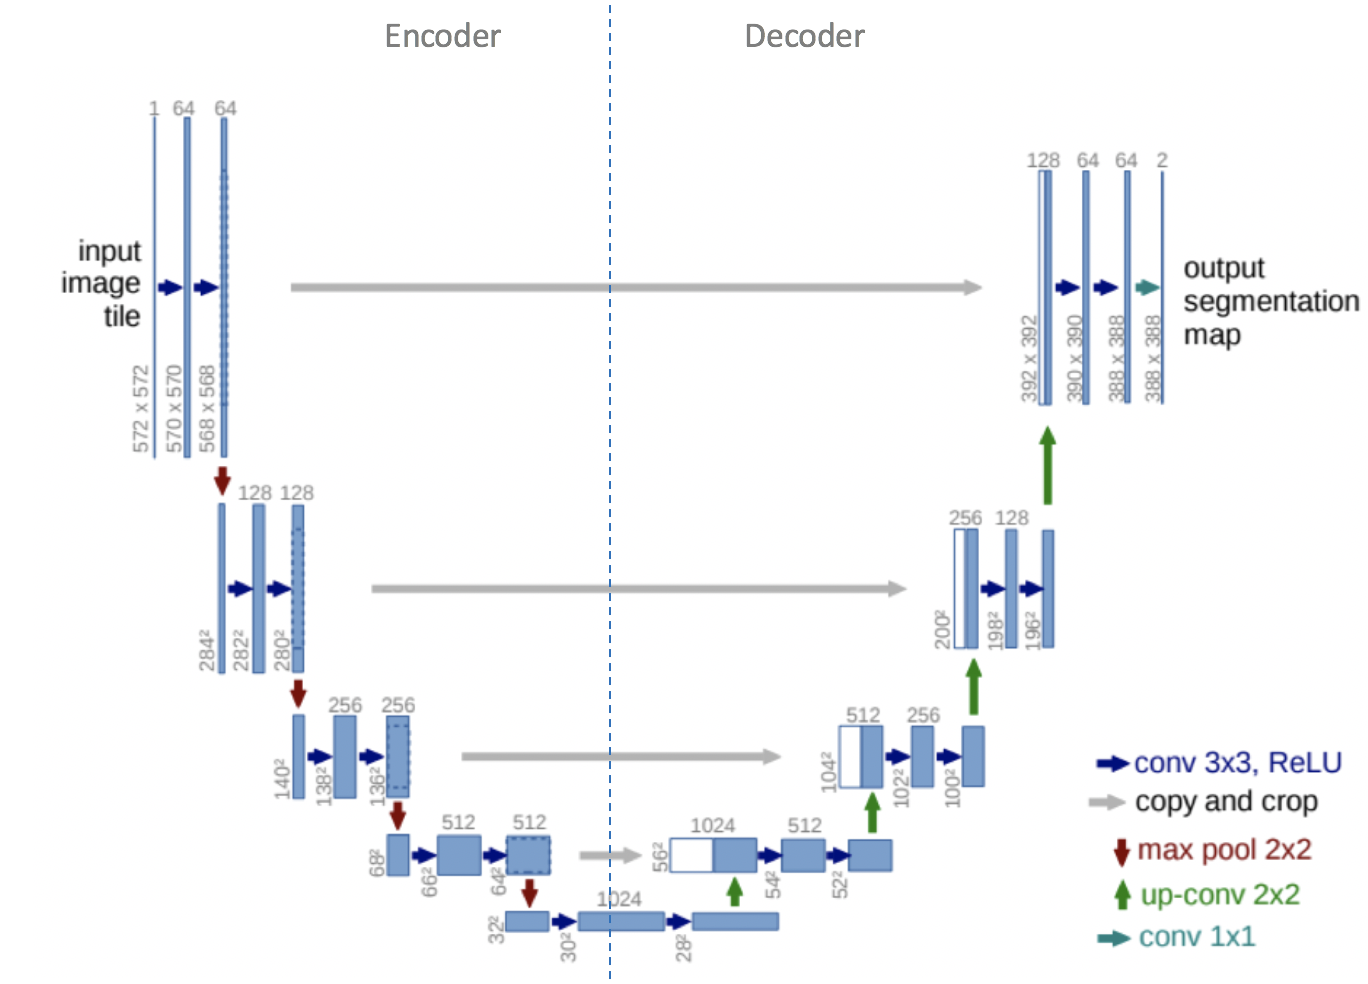
\includegraphics[width=.9\linewidth]{figure/unet.png}
\end{minipage}%
\begin{minipage}{.5\textwidth}
  \centering
  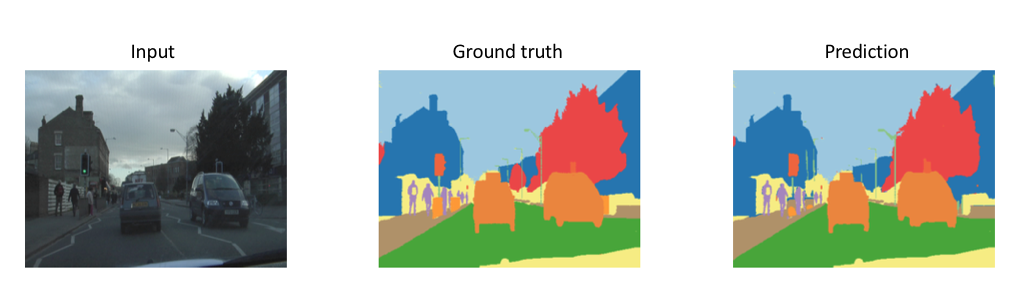
\includegraphics[width=.9\linewidth]{figure/semantic_segmentation.png}
\end{minipage}
\caption\tiny{U-Net, Ronneberger et al. MICCAI 2015}
\end{figure}

\end{vbframe}

\begin{vbframe}{Semantic Segmentation}

The goal of image captioning is to convert a given input image into a natural language description.

\begin{figure}
\centering
\begin{minipage}{.65\textwidth}
  \centering
  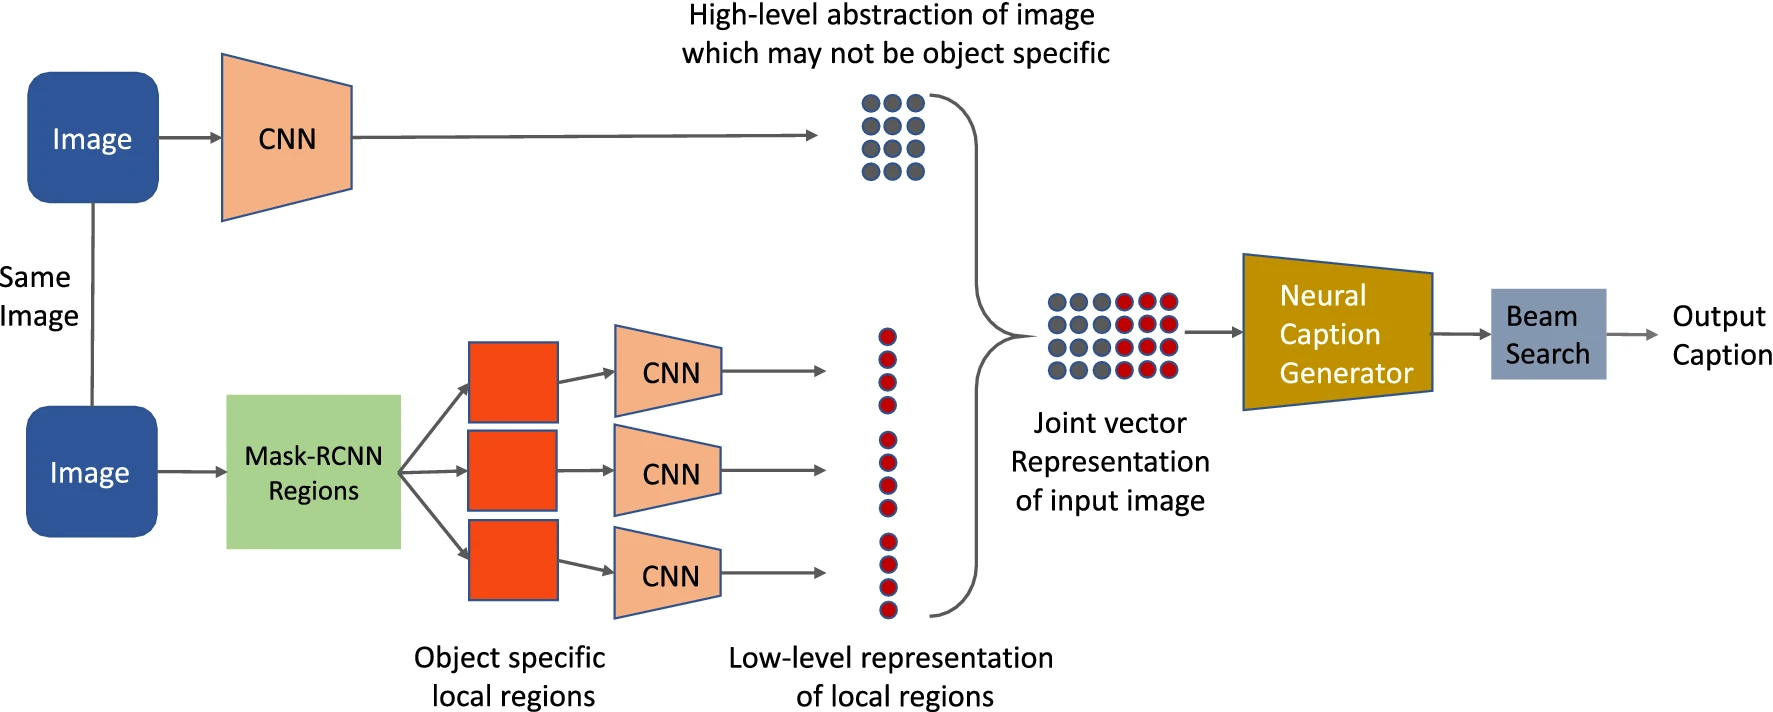
\includegraphics[width=.9\linewidth]{figure/caption_generation.png}
\end{minipage}%
\begin{minipage}{.35\textwidth}
  \centering
  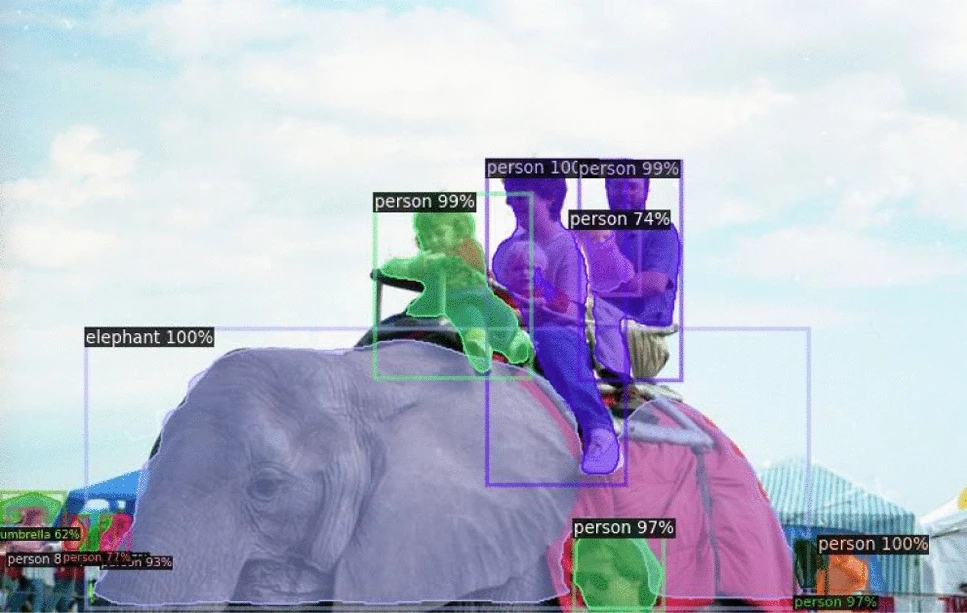
\includegraphics[width=.9\linewidth]{figure/example_sample_generation.png}
\end{minipage}
\caption\tiny{Caption generation with augmented visual attention by Biswas et al.2020}
\end{figure}

\end{vbframe}


%%%%%%%%%%%%%%%%%%%%%%%%%%%%%%%%%%%%%%%%%%%%%%%%%%%%%%%%%%%%%%%%%%
  %%%%%%%%%%%%%%%%%%%%%%%%%%%%%%%%%%%%%%%%%%%%%%%%%%%%%%%%%%%%%%%%%%
\endlecture
\end{document}